
\subsection{Personal Histories}

The following sections will feature many of the same figures;
here we will introduce them so their interleaving stories may be told
uninterrupted in the following sections.
Readers unfamiliar with the history of Unix may find unfamiliar terms in these
personal accounts; these will be discussed in the following sections after
our characters have been introduced.

\subsubsection{Doug McIlroy, Joined 1958}

Douglas McIlroy was born in Fishkill, New York.
His father worked in electrical engineering and spent time at
MIT and ended his career at Cornel, having contributed to the RADAR effort in World War II.
His father collected maps, and Doug grew an interest in maps himself.
One day, while ill in bed with chicken pox, his father assigned him the task of drawing
a dam on a USGS map, and showing which regions would be inundated by the dam
\cite{doug_mcilroy_oral_history_2019}.
His mother, too, had a master's degree in physics from the University of Rochester,
which was very unusual at the time. She was forced to audit some of her classes there,
because "women can't take this class! But you can sit in on it, if you want."
Thus he was raised in an engineering-minded household.

Barbara, his wife, also studied mathematics and faced discouragement similar to his mother's.
They ended up meeting at the laboratory, where Doug recalled that some figures at the labs sought
to improve the situation for women, specifically Bernie Holbrook.

Doug joined Bell Labs in 1958 and shortly thereafter earned his
PhD in applied mathematics from MIT.
McIlroy became head of the Computing Techniques Research department in 1965, and he's regarded
as one of the most brilliant members of the staff by key members that readers may be more familiar with.

He is described by nearly everyone at the Bell Labs Computing Research Center
(who wrote or spoke about their time there)
as the most brilliant member of that team that no one has heard of
\cite{kernighan_interviews_thompson_2019}; Ken Thompson described him as
"the smartest one of all of us and the least remembered or written down of all of us."

He was relatively hands-off as a manager, preferring to peek into his employees' offices
with suggestions or interesting problems and wait for the employees to let \textit{him} know
what needed to be done, rather than assigning tasks directly.
His employees respected his tasted in technical and personal matters,
as Brian Kernighan describes\cite{kernighan_unix:_2020}:

\begin{quotation}
	Unix might not have existed, and certainly
	would not have been as successful, without Doug's good taste and sound
	judgment of both technical matters and people.
\end{quotation}

\begin{figure}
	\centering
	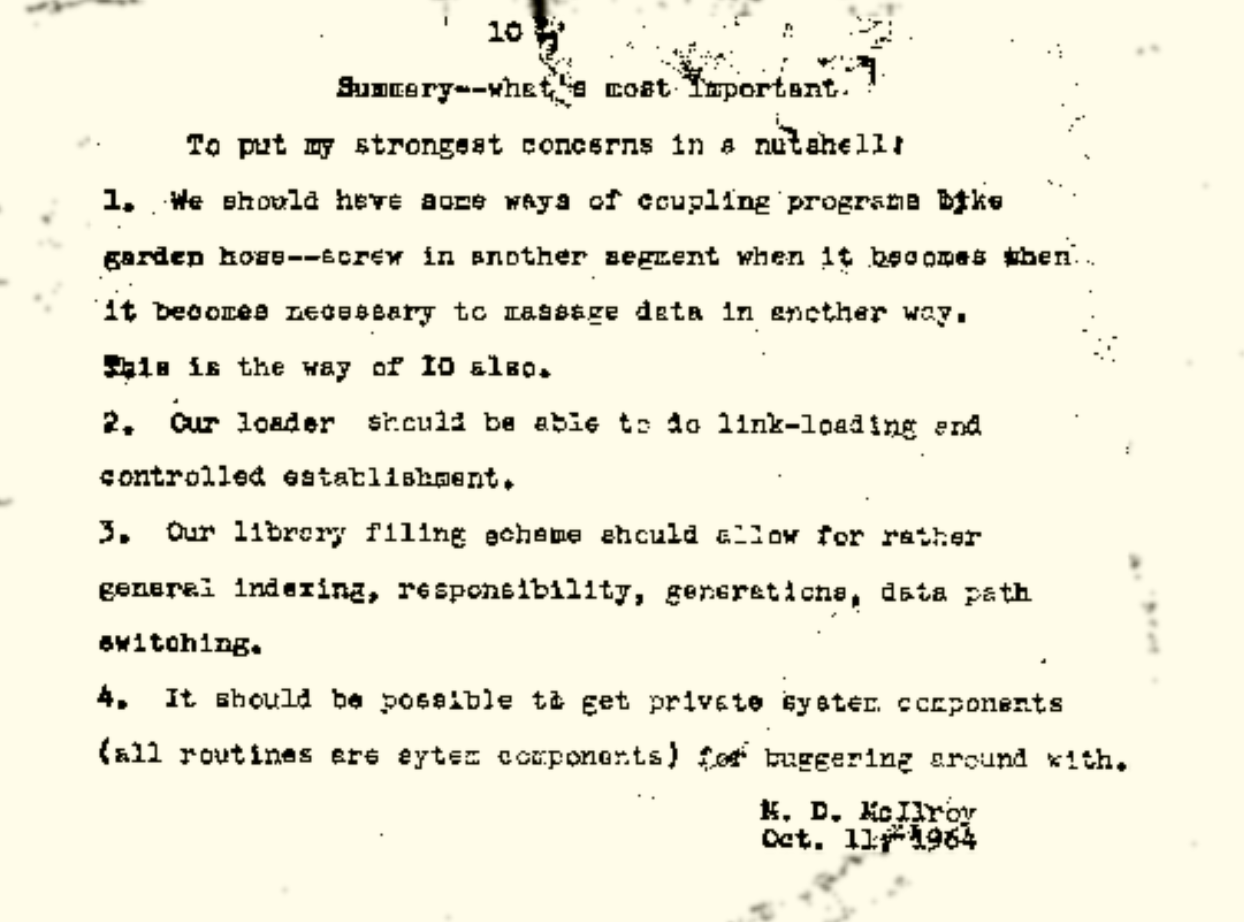
\includegraphics[width=0.7\textwidth]{resource/software/unix/doug-1964-pipes.png}
	\caption{Doug McIlroy's 1964 memo proposing Unix pipes\cite{doug_mcilroy_origin_of_unix_pipes_1964}.}
	\label{fig:unix-pipes-mcilroy-memo}
\end{figure}

In 1964, he circulated a memo which led to Unix pipes\cite{doug_mcilroy_origin_of_unix_pipes_1964}
(see \ref{fig:unix-pipes-mcilroy-memo}) though it took him quite a while to convince
Ken Thompson that he really ought to implement them.
Aside from pipes, he wrote many common Unix utilites we still use today, like
\texttt{diff}, \texttt{sort}, \texttt{join}, \texttt{tr}, \texttt{echo}, \texttt{tee}, and \texttt{spell}.

He hired Alfred Aho in 1967\cite{aho_oral_history_2022}:

\begin{quotation}
	I was interviewed by a department head by the name of Doug McIlroy. He was an applied
	mathematician from MIT. He had been at Bell Labs for a few years before me. Amongst other things, he
	had co-invented macros for programming languages and he's also in this class of one of the smartest
	people I've ever met.
\end{quotation}

\subsubsection{Ken Thompson, Joined 1966}

\todo{Ken's oral history is rich and includes fun stories about how he was recruited to the labs.}

\subsubsection{Dennis Ritchie, Joined 1967}


\subsubsection{Jeffrey Ullman, Joined 1967}

\todo{This section can be shorter since Ullman went back to Princeton and only consulted at the lab part-time.}

\subsubsection{Alfred Aho, Joined 1967}

Alfred grew up in a Finnish household, and when he showed up to Kindergarten,
he couldn't speak any English.
In his first report card, the teacher told his parents that "Al can't speak any English!",
and in the next report card, the teacher said reported that "Al speaks \textit{too much} English!";
so he learned it relatively late and became quite a social kid.
Alfred played music all throughout his childhood, and the schools he went to
as a kid had quite good musical programs.
He went to University of Toronto for undergraduate school and continued playing
the violin all through his years at Bell Labs. He was an only child. He had a
proclivity not only for music but for mathematics and reading science fiction.

After finishing his undergraduate degree in Toronto in engineering physics,
he got a masters and then PhD
from Princeton University in electrical engineering and computer science,
completing the latter in 1967.
At Princeton took a course from John Hopcroft on computer science theory with a heavy emphasis on
automata and language theory, which sparked his long-lasting interest in formal languages.
His PhD thesis was on extending the theory of context-free grammars, an area of
expertise that would serve him well at the Labs.

One of the fist people he met at Princeton was Jeffrey Ullman, who had also recently
started there, beginning a long-term friendship and collaboration between the two
\cite{aho_oral_history_2022}:

\begin{quotation}
	One of the first people that I met at Princeton was a Columbia graduate by the name of Jeffrey
	Ullman. He had just gotten his undergraduate degree from Columbia University and also had come to
	study digital systems in the EE department at Princeton. So, he and I became close friends. When we
	graduated from Princeton, we both joined the newly formed Computing Sciences Research Center at Bell
	Labs. There we developed a lifelong collaboration on subjects ranging from algorithms, programming
	languages, to the very foundations of computer science. I was very fortunate to have met some of the
	greatest people in the field and to have gotten to know them and work with them.
\end{quotation}

His PhD advisor was John Hopcroft, whom he would also continue to work with for a long time.
He told Alfred to "find his own research problem," and he turned to his interest in
programming languages and compilers.
He was always very keen on precision; he wanted to use precise terms and he would
press even his own friends to be very precise in their informal discussions, and
this acuity for precision extended to his thesis, which was on the very precise
understanding of the \textit{syntax} and the \textit{semantics} of programming languages.
Alfred would contribute his deep understanding of the theory of automata and programming
languages to the Labs, where there were many other brilliant people who were more practical
and lacked familiarity with the literature.
In 1967 his good friend Jeffrey Ullman had started working at Bell Labs, and a few months
after starting there, Alfred interviewed there.
He was interviewed by Doug McIlroy, who hired him.
For some time, he and Jeffrey worked together at the Labs, but Jeffrey had wanted to
spend more time in academia than Alfred, so he returned to Princeton's electrical
engineering department, but continued to consult at Bell Labs one day a week.
Thus the two continued to work together.
Alfred described their collaboration at Bell Labs:

\begin{quotation}
	He stayed at Bell Labs for a few years and went to Princeton University where he
	joined the faculty of the electrical engineering department, but he would come and spend one day a
	week consulting at Bell Labs. His consulting stint, he would come Fridays and sit in my office
	all day. The conversations that we'd have would range over all sorts of topics, and sometimes he'd
	mentioned that he was working on a problem with a colleague at Princeton, and after describing the
	problem, I might say, "You're kidding," and he said, "Oh, you're right. The solution is obvious,
	isn't it?" I don't know whether I would say dynamic programming or whatever, but several papers
	came out of this intense collaboration, and we got to the point where we could communicate with just
	a few words. We had a very large, shared symbol table.
	\cite{aho_oral_history_2022}
\end{quotation}

Ken Thompson joined the labs several months before the two of them to
start working on Multics, and had developed a plethora of tools based on
regular expressions, such as \texttt{grep}.
This combined with the \texttt{ED} and \texttt{QED} editors that came from MIT
and were shipped with Multics sparked Alfred's interest in regular expressions.

Aho is probably best known for the textbooks he co-authored with his friend Jeffrey,
colloquially known as \textit{The Dragon Book} (\citetitlecite{the_dragon_book_aho_ullman_sethi_1986})
and his book with John Hopcroft on algorithms, \citetitlecite{aho_hopcroft_algorithms_1974}.

\subsubsection{Brian Kernighan, Joined 1969}

\subsubsection{David McQueen, Joined 1981}

David didn't start working at the labs until much later than the others in this section
and he primarily worked on his own, unlike the others mentioned in this section.
Because of his work on Meta Language and type theory, we include some of his personal history here
as well.
